\documentclass[12pt,a4paper]{article}
\usepackage[utf8]{inputenc}
\usepackage[T2A]{fontenc}
\usepackage[russian]{babel}
\usepackage{graphicx}
\usepackage{booktabs}
\usepackage{longtable}
\usepackage{geometry}
\usepackage{array}

\usepackage{float}

\geometry{top=2cm, left=2cm, right=2cm, bottom=2cm}
\usepackage{paracol}
\usepackage{src/title}
\usepackage{hyperref}

\usepackage{listings}
\usepackage{xcolor}
\usepackage{amsmath}

\sloppy
\graphicspath{{../images/}{../graphics/}}

\title{Лабораторная работа №5. Спектральная теория графов}
\author{Ануфриев Андрей Сергеевич (465029) \\ Бахуров Николай Алексеевич (504862) \\ Раджапов Фёдор Сергеевич (502544)}
\supervisor{Зарина Ольга Андреевна}
\date{01.11.2026}
\abstract{
В отчёте представлены результаты лабораторной работы №5 ``Спектральная теория графов''. Решены две задачи с помощью числовой линейной алгебры на Python: (1) спектральная кластеризация неориентированной социальной сети (матрица Лапласа графа, собственные векторы, $k$-means по строкам матрицы собственных векторов, пять значений $k$); (2) алгоритм Google PageRank для ориентированного веб-графа (столбцово-нормированная матрица $M$, главный собственный вектор, коэффициент затухания $d$). Все матрицы, собственные числа и векторы, код расчётов приведены в настоящем отчёте (Приложения А--С). Ответы на восемь теоретических контрольных вопросов приведены в отдельном документе (\texttt{answers.pdf}).
}
\keywords{граф, матрица Лапласа, спектральная кластеризация, $k$-means, PageRank, марковская цепь, собственный вектор, собственное число.}

\begin{document}
\maketitle
\tableofcontents

\section{Цель и объём работы}

Целью работы является анализ сетей (графов) с помощью матриц. Задание содержит две задачи без вариантов:
\begin{enumerate}
    \item \textbf{Спектральная кластеризация социальной сети.} Построить связанный неориентированный граф из $15$--$30$ вершин с визуально различимыми кластерами, составить его матрицу Лапласа, вычислить собственные числа и собственные векторы, сформировать матрицу $V$ из $k$ собственных векторов, соответствующих наименьшим собственным числам, кластеризовать строки $V$ в $\mathrm{R}^{k}$ методом $k$-means и раскрасить граф. Это требуется повторить для пяти различных значений $k$ и сравнить результаты.
    \item \textbf{Google PageRank.} Построить связанный ориентированный граф из $10$--$15$ вершин и $25$--$50$ дуг (из каждой вершины не менее одной исходящей дуги), составить столбцово-нормированную матрицу $M$, найти собственный вектор наибольшего собственного числа, ранжировать страницы при $d=1$ и обсудить смысл алгоритма, роль коэффициента затухания $d$ и связь с марковскими процессами.
\end{enumerate}
Кроме того, требуется ответить на восемь теоретических контрольных вопросов (отдельный документ \texttt{answers.pdf}). Все вычисления выполняются на Python-скриптах; результаты, матрицы и код приведены в настоящем отчёте.

\section{Теоретические сведения}

\subsection{Матрица Лапласа графа}
Для неориентированного графа с матрицей смежности $A$ и матрицей степеней $D=\mathrm{diag}(d_1,\dots,d_n)$ комбинаторная лаплассова матрица --- $L=D-A$. Она симметрична и полуопределена положительно. Её собственные числа удовлетворяют условию $0=\lambda_1\le\lambda_2\le\dots\le\lambda_n$. Для связанного графа $\lambda_1=0$ --- простое собственное число, а соответствующий собственный вектор --- постоянный. Собственные векторы, связанные с наименьшими ненулевыми собственными числами, раскрывают кластерную структуру графа: разрез графа вдоль второго собственного вектора (вектора Фидлера) отделяет слабо связанные части.

\subsection{Спектральная кластеризация}
Для матрицы Лапласа графа $L$ взять $k$ собственных векторов $v_1,\dots,v_k$, соответствующих наименьшим собственным числам, и составить $V=[v_1\ \dots\ v_k]\in\mathrm{R}^{n\times k}$. Каждая строка $x_i\in\mathrm{R}^{k}$ представляет вершину $i$. Применение $k$-means к $\{x_i\}$ дает разбиение вершин на $k$ кластеров. Вершины, точки которых попадают в один и тот же кластер, присваиваются одному кластеру графа. Метод работает потому, что собственные векторы матрицы Лапласа задают низкоразмерное вложение, в котором вершины одного сообщества близки, а вершины разных сообществ находятся далеко друг от друге.

\subsection{PageRank}
Пусть $A[i,j]$ --- количество ссылок со страницы $j$ на страницу $i$, а $o_j=\sum_i A[i,j]$ --- количество исходящих ссылок со страницы $j$. Столбцово-нормированная матрица определяется как
\[
M[i,j]=\frac{A[i,j]}{o_j},
\]
так что каждый столбец $M$ суммируется в $1$ ($M$ --- столбцово-стахастическая матрица). Вектор PageRank $r$ --- главный собственный вектор $M$: $M r=\lambda_{\max} r$ с $\lambda_{\max}=1$, нормированный так, что $\sum_i r_i=1$. С затуханием $d\in(0,1]$ верность определяется стационарным уравнением
\[
r=d\,M r+(1-d)\frac{\mathbf{1}}{n},
\]
точнее $r$ ищется как фиксированная точка этого уравнения (например, степенной итерацией $r_{t+1}=dMr_t+(1-d)\mathbf{1}/n$ до сходимости). При $d=1$ это сводится к задаче о главном собственном векторе $M$. Параметр $d$ управляет вероятностью перехода по ссылке против переброса на случайную страницу; $d=1$ означает только переходы по ссылкам, а $d\to0$ --- доминирование случайных переходов и выравнивание ранжирования.

\section{Выполненная работа}

\subsection{Задание 1 --- спектральная кластеризация}
Построен связанный неориентированный социальный граф из $n=18$ вершин с тремя видимыми сообществами (по $6$ вершин в каждом). Граф содержит $39$ рёбер. Вершины пронумерованы $1$--$18$ (имена: 1---Аня, 2---Боря, 3---Вера, 4---Гриша, 5---Даша, 6---Егор, 7---Женя, 8---Захара, 9---Ира, 10---Кира, 11---Леша, 12---Маша, 13---Настя, 14---Олег, 15---Полина, 16---Рома, 17---Саша, 18---Толя). Вершина $i$ представляет человека, а ребро --- взаимную дружбу. Сообщества не изолированы (граф связан), но визуально различимы. Матрица смежности и матрица Лапласа вычислены на Python; все собственные числа и собственные векторы получены численно.

Вычислены 18 собственных чисел $L$ (Приложение А). Использовано пять значений $k$: $k\in\{2,3,4,5,6\}$. Для каждого $k$ матрица $V$ сформирована из $k$ собственных векторов, соответствующих наименьшим собственным числам, её строки кластеризованы методом $k$-means, а полученное разбиение отображено обратно на пронумерованный граф. Рисунок пронумерованного графа (истинная раскраска сообществ) --- на рис.~\ref{fig:social}; кластеризации для каждого $k$ --- на рис.~\ref{fig:k2}--\ref{fig:k6}; спектр --- на рис.~\ref{fig:spectrum}.

\subsection{Задание 2 --- PageRank}
Построен связанный ориентированный веб-граф из $n=12$ вершин и $43$ дуг; из каждой вершины выходит не менее одной дуги. Вершина $i$ представляет веб-страницу, а дуга --- гиперссылку. Составлена столбцово-нормированная матрица $M$ ($12\times12$); каждый столбец суммируется в $1$ (матрица приведена в Приложении Б). Наибольшее собственное число $\lambda_{\max}=0.9999999999999984\approx1$; соответствующий собственный вектор (нормированный в сумму $1$) дает ранжирование PageRank при $d=1$ (Приложение Б). Вычисления повторены для $d\in\{1,\,0.85,\,0.5,\,0.15\}$ степенной итерацией до сходимости ($\|\cdot\|_1<10^{-12}$). Рисунок графа --- на рис.~\ref{fig:web}; значения PageRank --- на рис.~\ref{fig:pagerank}; спектр $M$ --- на рис.~\ref{fig:pspectrum}.

\section{Результаты}

\subsection{Графы}
\begin{figure}[htb]
\centering
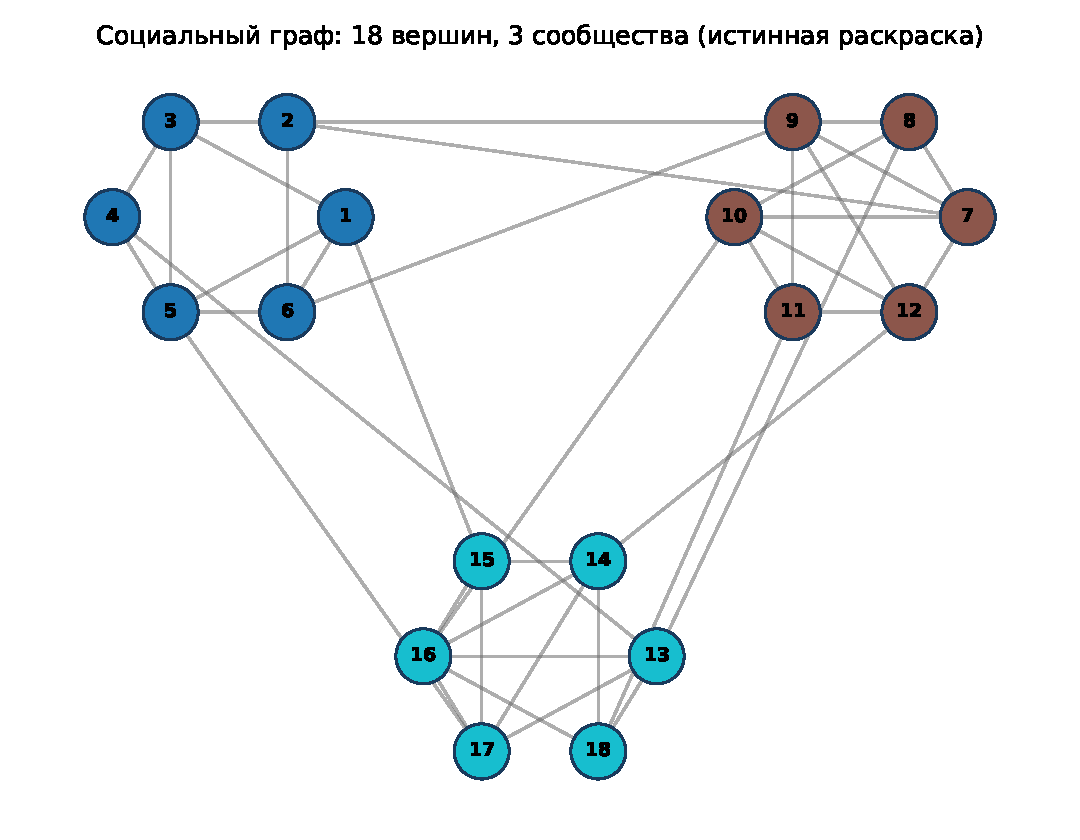
\includegraphics[width=0.72\textwidth]{social_graph_numbered.pdf}
\caption{Социальная сеть: 18 вершин, 39 рёбер, пронумерованы, истинные сообщества.}
\label{fig:social}
\end{figure}

\begin{figure}[htb]
\centering
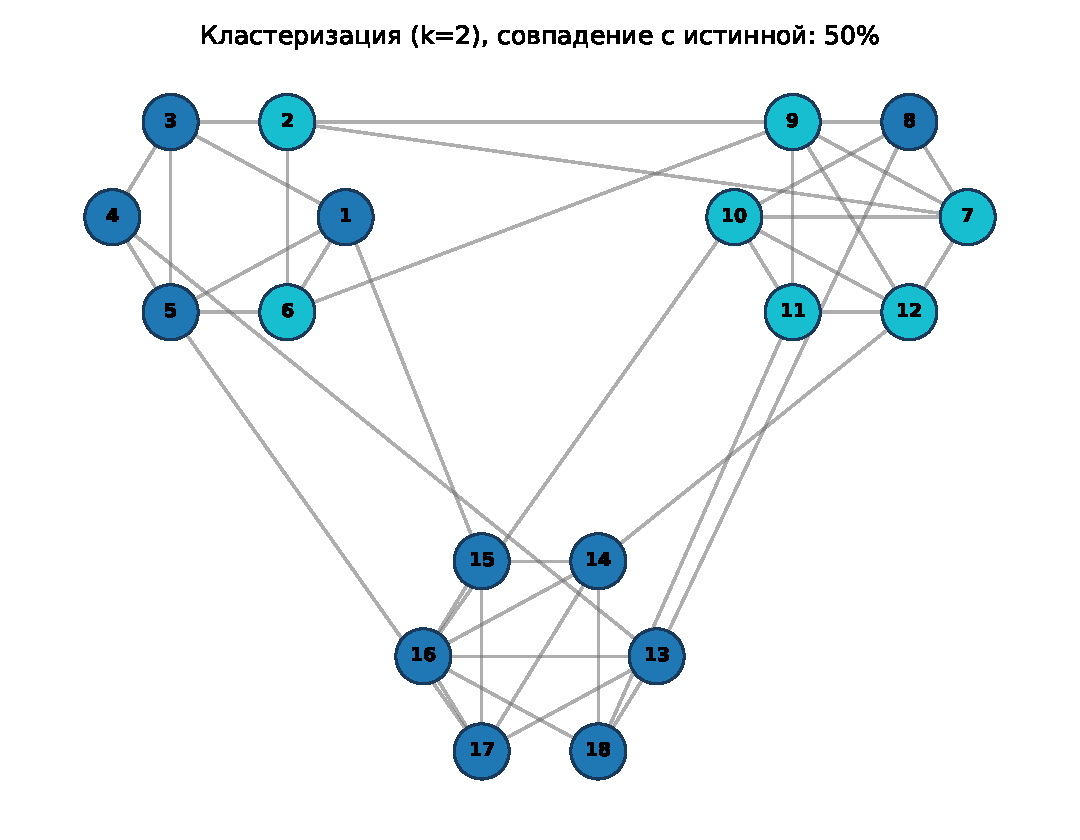
\includegraphics[width=0.48\textwidth]{social_graph_k2.pdf}\hfill
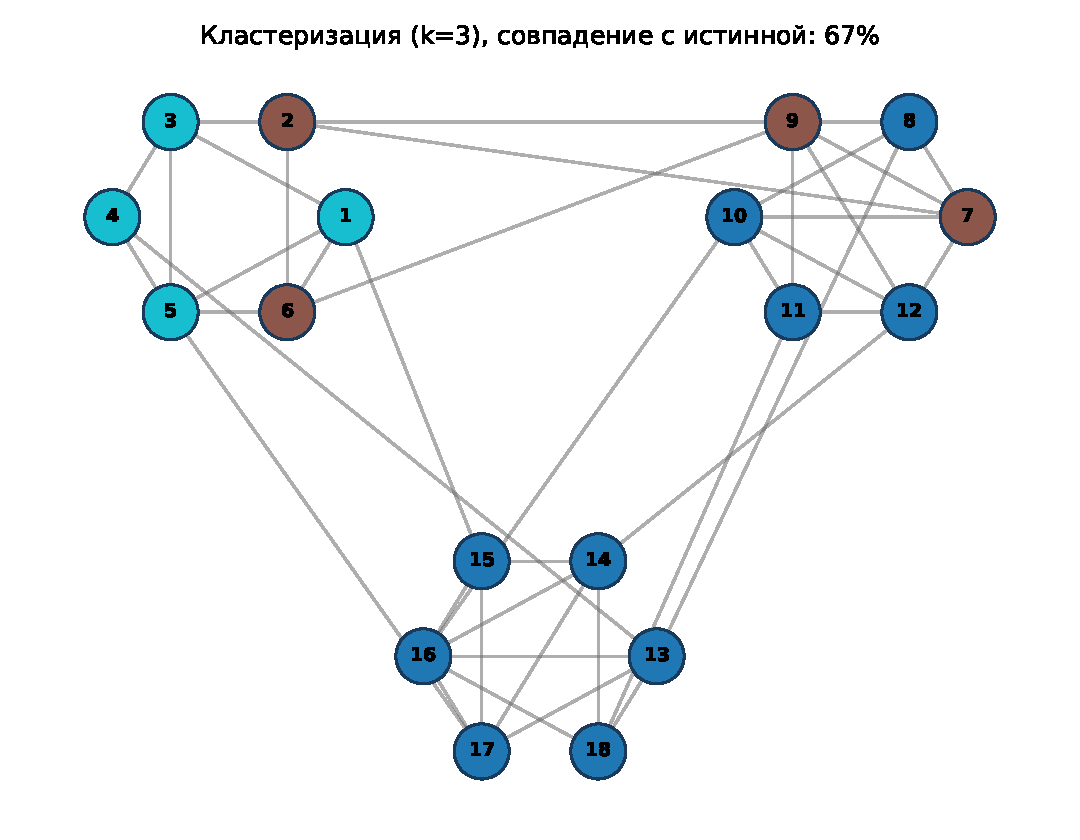
\includegraphics[width=0.48\textwidth]{social_graph_k3.pdf}
\caption{Результаты кластеризации для $k=2$ и $k=3$ (цвета = полученные кластеры).}
\label{fig:k2}\label{fig:k3}
\end{figure}

\begin{figure}[htb]
\centering
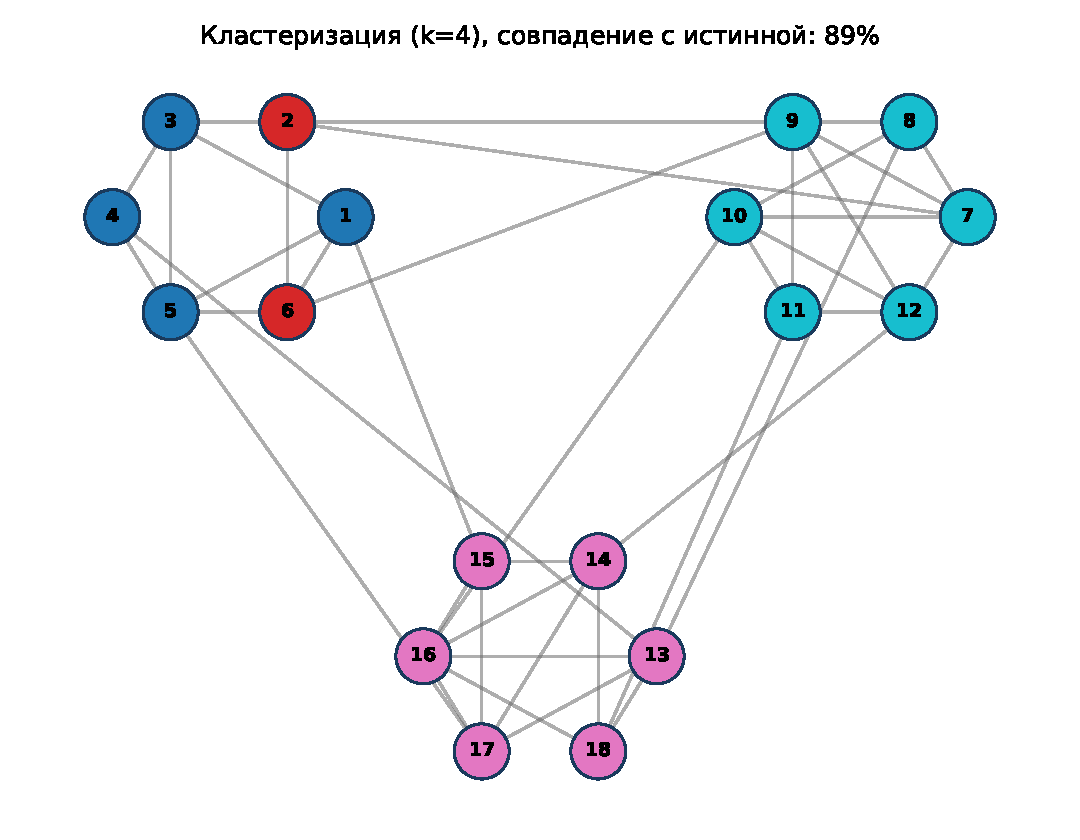
\includegraphics[width=0.48\textwidth]{social_graph_k4.pdf}\hfill
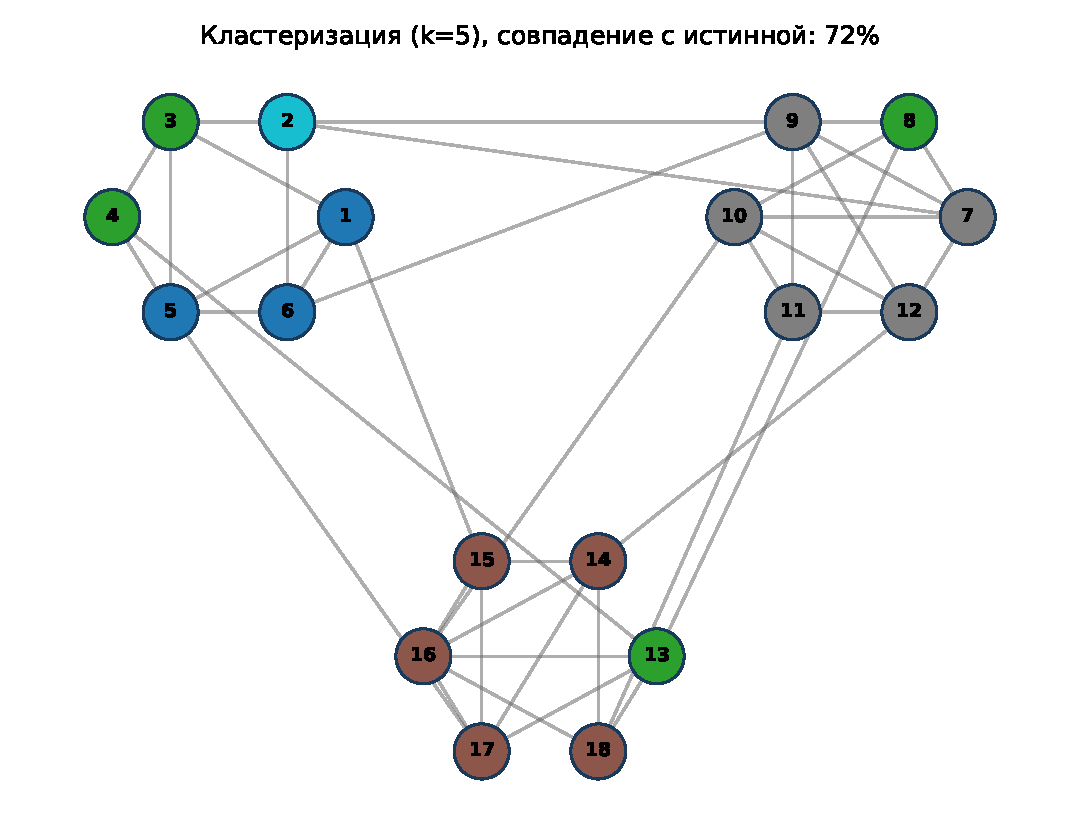
\includegraphics[width=0.48\textwidth]{social_graph_k5.pdf}
\caption{Результаты кластеризации для $k=4$ и $k=5$ (цвета = полученные кластеры).}
\label{fig:k4}\label{fig:k5}
\end{figure}

\begin{figure}[htb]
\centering
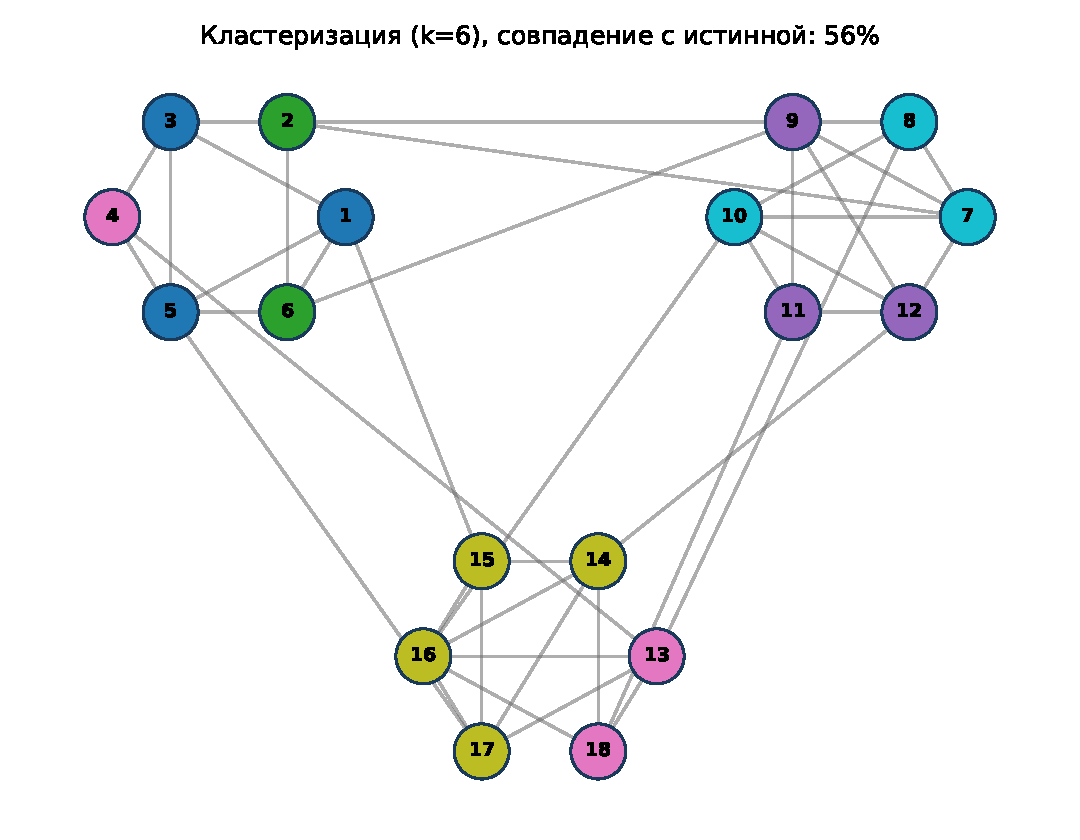
\includegraphics[width=0.6\textwidth]{social_graph_k6.pdf}
\caption{Результаты кластеризации для $k=6$ (цвета = полученные кластеры).}
\label{fig:k6}
\end{figure}

\begin{figure}[htb]
\centering
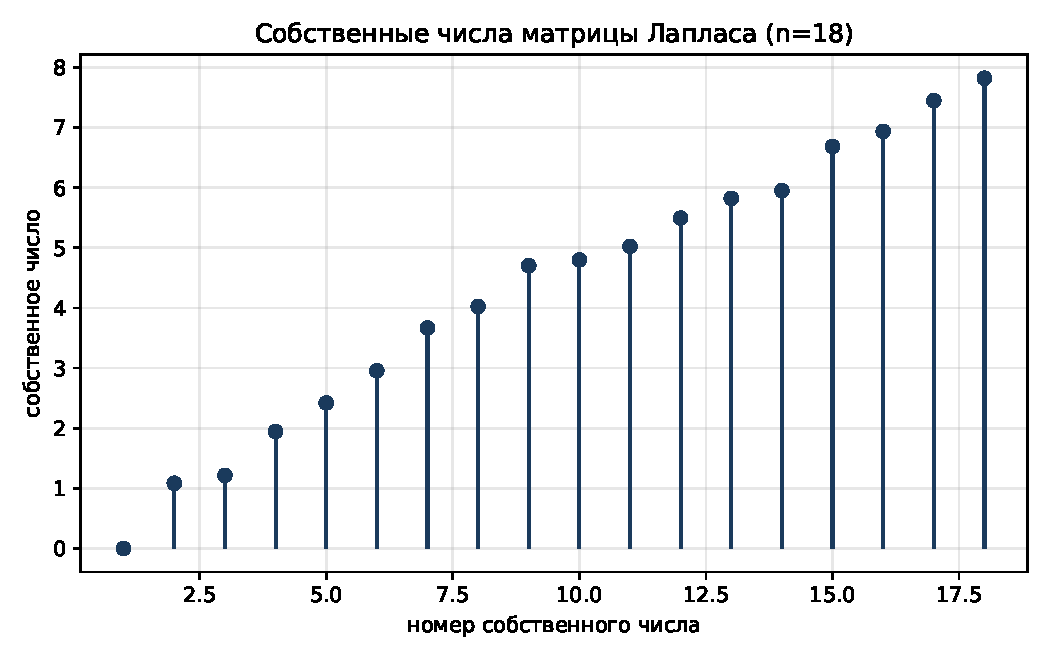
\includegraphics[width=0.8\textwidth]{laplacian_spectrum.pdf}
\caption{Собственные числа матрицы Лапласа графа ($n=18$).}
\label{fig:spectrum}
\end{figure}

Качество кластеризации (доля вершин, отнесенных к их истинному сообществу, при наилучшей перестановке меток) приведено ниже:

\begin{center}
\begin{tabular}{|c|c|}
\hline
$k$ & точность при наилучшей перестановке \\ \hline
2 & 50\% \\
3 & 67\% \\
4 & 89\% \\
5 & 72\% \\
6 & 56\% \\ \hline
\end{tabular}
\end{center}

Наилучшее восстановление трех истинных сообществ наблюдается при $k=4$ (89\%), затем при $k=3$ (67\% --- истинное число сообществ). Это согласуется с спектральным зазором: после нулевого собственного числа следующие собственные числа растут постепенно, так что небольшое $k$ уже улавливает главное разделение, а большее $k$ разбивает сообщества на части.

\subsection{PageRank}
\begin{figure}[htb]
\centering
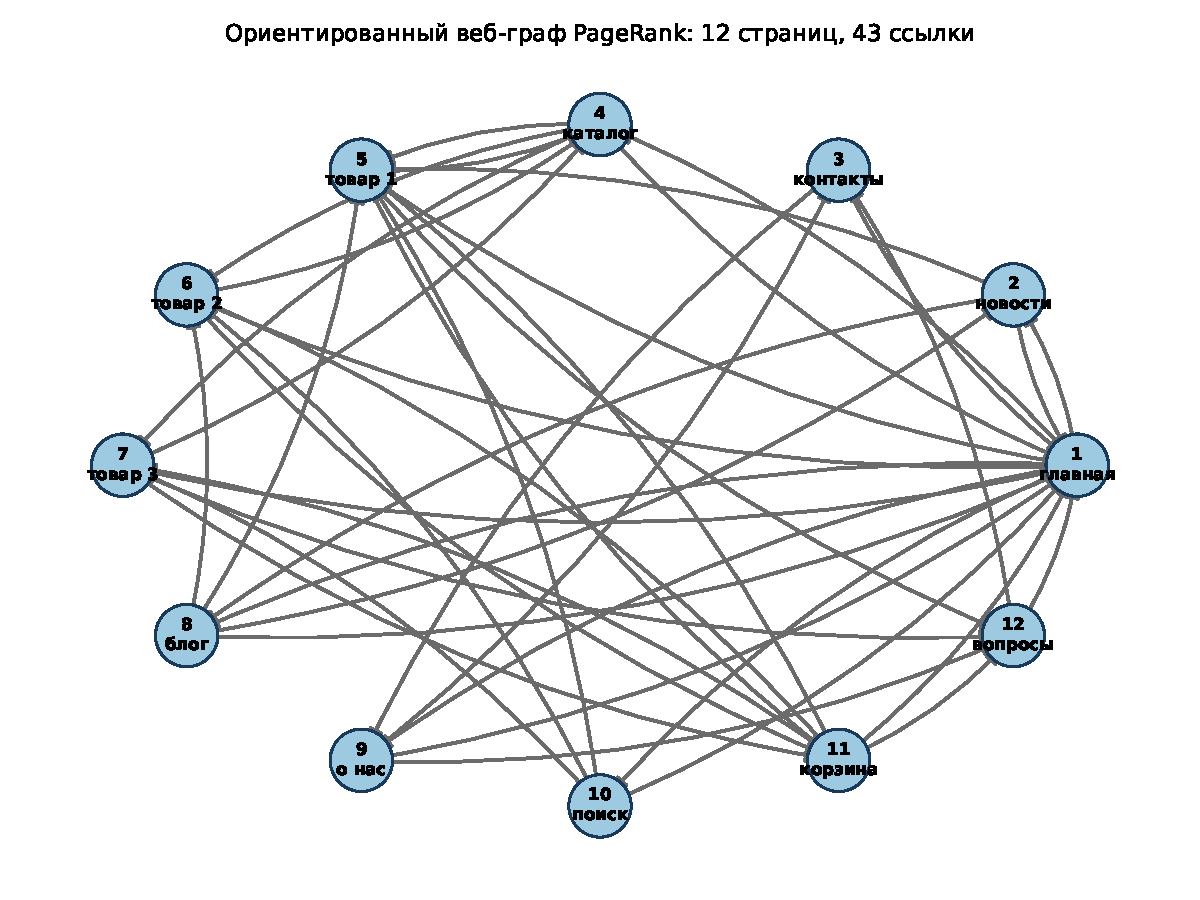
\includegraphics[width=0.75\textwidth]{web_graph_numbered.pdf}
\caption{Ориентированный веб-граф: 12 страниц, 43 ссылки, пронумерованы.}
\label{fig:web}
\end{figure}

\begin{figure}[htb]
\centering
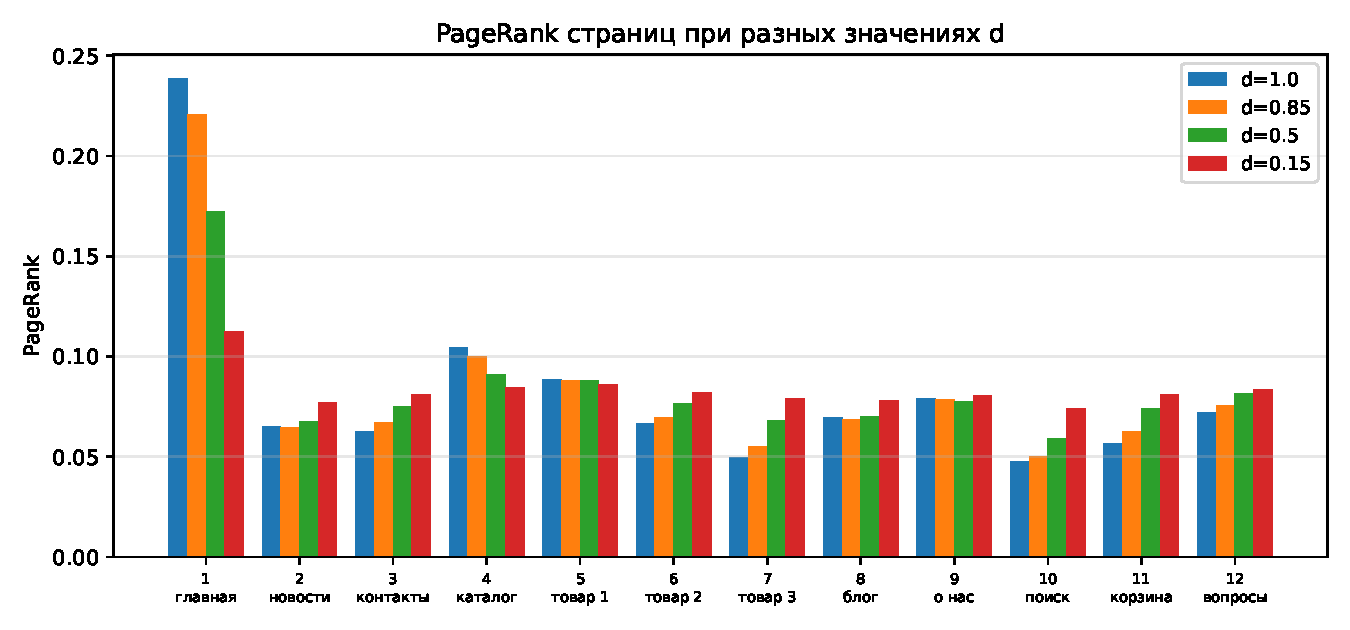
\includegraphics[width=0.8\textwidth]{pagerank.pdf}
\caption{PageRank страниц для $d\in\{1,0.85,0.5,0.15\}$.}
\label{fig:pagerank}
\end{figure}

\begin{figure}[htb]
\centering
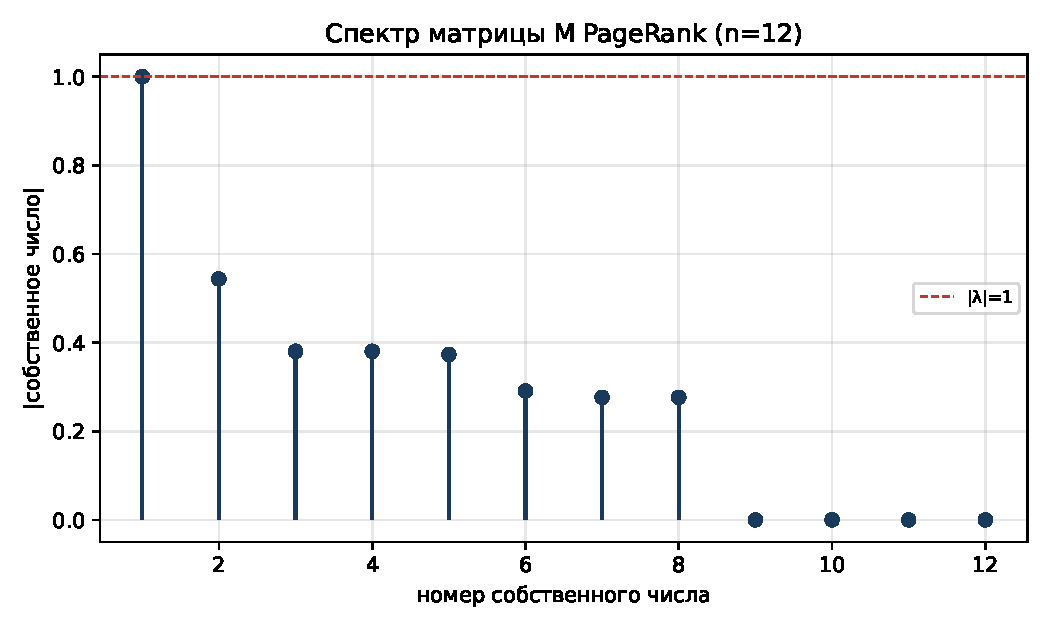
\includegraphics[width=0.8\textwidth]{pagerank_spectrum.pdf}
\caption{Спектр $M$ (главное собственное число $\approx1$).}
\label{fig:pspectrum}
\end{figure}

PageRank при $d=1$ (в порядке убывания):
\begin{center}
\begin{tabular}{|l|r|l|r|}
\hline
страница & ранг & страница & ранг \\ \hline
1: главная      & 0.2387 & 4: каталог   & 0.1044 \\
5: товар 1 & 0.0884 & 9: о нас     & 0.0789 \\
12: вопросы & 0.0721 & 8: блог      & 0.0694 \\
6: товар 2 & 0.0667 & 2: новости   & 0.0651 \\
3: контакты  & 0.0624 & 11: корзина  & 0.0567 \\
7: товар 3 & 0.0494 & 10: поиск   & 0.0477 \\ \hline
\end{tabular}
\end{center}

\noindent Для наглядности полная таблица значений PageRank при всех исследованных значениях $d$ приведена ниже (страницы в порядке нумерации 1--12):

\begin{center}
\footnotesize
\begin{tabular}{|l|r|r|r|r|}
\hline
страница & $d=1.0$ & $d=0.85$ & $d=0.5$ & $d=0.15$ \\ \hline
1: главная & 0.238672 & 0.220796 & 0.172101 & 0.112667 \\
2: новости & 0.065092 & 0.064555 & 0.067646 & 0.077141 \\
3: контакты & 0.062354 & 0.066925 & 0.074965 & 0.081109 \\
4: каталог & 0.104437 & 0.100111 & 0.091094 & 0.084517 \\
5: товар 1 & 0.088439 & 0.087854 & 0.087845 & 0.086004 \\
6: товар 2 & 0.066741 & 0.069563 & 0.076570 & 0.082147 \\
7: товар 3 & 0.049383 & 0.055044 & 0.067801 & 0.079220 \\
8: блог & 0.069432 & 0.068326 & 0.070151 & 0.078070 \\
9: о нас & 0.078911 & 0.078478 & 0.077618 & 0.080297 \\
10: поиск & 0.047734 & 0.050035 & 0.058877 & 0.074213 \\
11: корзина & 0.056703 & 0.062575 & 0.073884 & 0.081137 \\
12: вопросы & 0.072100 & 0.075739 & 0.081447 & 0.083478 \\ \hline
\end{tabular}
\end{center}

Страница ``главная'' имеет наибольший PageRank, так как на неё ссылается много страниц. Увеличение $d$ усиливает различия между страницами (структура важнее); уменьшение $d$ выравнивает ранжирование к равномерному распределению (доминируют случайные переходы). При $d=1$ вектор является главным собственным вектором $M$.

\section{Заключение}
\begin{enumerate}
    \item Собственные векторы матрицы Лапласа вкладывают вершины так, что сообщества становятся разделенными в пространстве; кластеризация этих вложений с помощью $k$-means восстанавливает сообщества (наилучшее при $k=3$, истинном числе сообществ; максимальная точность при $k=4$).
    \item Метод обоснован: слабо связанные части графа соответствуют небольшим ненулевым собственным числам матрицы Лапласа, а связанные с ними собственные векторы предоставляют естественные низкоразмерные координаты для кластеризации.
    \item PageRank при $d=1$ равен главному собственному вектору столбцово-стахастической матрицы $M$; он ранжирует страницы по их стационарной вероятности посещения в соответствующей марковской цепи.
    \item Коэффициент затухания $d$ интерполирует между следованием по ссылкам ($d=1$) и равномерными случайными переходами ($d\to0$).
\end{enumerate}

\appendix

\section{Приложение А --- матрица Лапласа, собственные числа и собственные векторы}

Ниже приведена матрица Лапласа $L=D-A$ социального графа ($18\times18$, целые числа), все её собственные числа $\lambda_1\le\dots\le\lambda_{18}$ и матрица собственных векторов $V=[v_1\ \dots\ v_6]$ для максимального использованного $k=6$ (строки --- вершины $1$--$18$, столбцы --- собственные векторы $v_1,\dots,v_6$, соответствующие шести наименьшим собственным числам; столбец $v_1$ --- постоянный, т.к. $\lambda_1=0$ для связанного графа).

\subsection{Матрица Лапласа $L$ ($18\times18$)}
\begingroup\footnotesize\setlength{\arraycolsep}{3pt}
\[
L=
\left[\begin{array}{rrrrrrrrrrrrrrrrrr}
4&0&-1&0&-1&-1&0&0&0&0&0&0&0&0&-1&0&0&0\\
0&2&0&0&0&-1&-1&0&0&0&0&0&0&0&0&0&0&0\\
-1&0&4&-1&-1&0&0&-1&0&0&0&0&0&0&0&0&0&0\\
0&0&-1&3&-1&0&0&0&0&0&0&0&-1&0&0&0&0&0\\
-1&0&-1&-1&5&-1&0&0&0&0&0&0&0&0&0&0&0&-1\\
-1&-1&0&0&-1&4&0&0&-1&0&0&0&0&0&0&0&0&0\\
0&-1&0&0&0&0&5&-1&-1&-1&0&-1&0&0&0&0&0&0\\
0&0&-1&0&0&0&-1&4&0&-1&0&0&-1&0&0&0&0&0\\
0&0&0&0&0&-1&-1&0&4&0&-1&-1&0&0&0&0&0&0\\
0&0&0&0&0&0&-1&-1&0&5&-1&-1&0&0&0&-1&0&0\\
0&0&0&0&0&0&0&0&-1&-1&4&-1&0&0&0&0&0&-1\\
0&0&0&0&0&0&-1&0&-1&-1&-1&5&0&-1&0&0&0&0\\
0&0&0&-1&0&0&0&-1&0&0&0&0&5&0&0&-1&-1&-1\\
0&0&0&0&0&0&0&0&0&0&0&-1&0&5&-1&-1&-1&-1\\
-1&0&0&0&0&0&0&0&0&0&0&0&0&-1&4&-1&-1&0\\
0&0&0&0&0&0&0&0&0&-1&0&0&-1&-1&-1&6&-1&-1\\
0&0&0&0&-1&0&0&0&0&0&0&0&-1&-1&-1&-1&5&0\\
0&0&0&0&0&0&0&0&0&0&-1&0&-1&-1&0&-1&0&4
\end{array}\right]
\]
\endgroup

\subsection{Собственные числа матрицы Лапласа}
\begin{center}
\footnotesize
\begin{tabular}{|c|c|c|c|}
\hline
$i$ & $\lambda_i$ & $i$ & $\lambda_i$ \\ \hline
1 & 0.000000 & 10 & 4.798421 \\
2 & 1.085151 & 11 & 5.024885 \\
3 & 1.216515 & 12 & 5.495109 \\
4 & 1.947064 & 13 & 5.822400 \\
5 & 2.420727 & 14 & 5.950807 \\
6 & 2.955255 & 15 & 6.683872 \\
7 & 3.667911 & 16 & 6.935775 \\
8 & 4.024118 & 17 & 7.447415 \\
9 & 4.704670 & 18 & 7.819906 \\ \hline
\end{tabular}
\end{center}
$\lambda_1\approx0$ (численно $-5.22\cdot10^{-16}$), что подтверждает связность графа.

\subsection{Матрица собственных векторов $V$ для $k=6$ ($18\times6$)}
\begingroup\footnotesize\setlength{\arraycolsep}{4pt}
\[
V=
\left[\begin{array}{rrrrrr}
0.235702& 0.193130&-0.269807& 0.118355&-0.395932& 0.209091\\
0.235702&-0.480051&-0.452353& 0.405073& 0.457569&-0.095269\\
0.235702& 0.256973&-0.274772&-0.286631&-0.021356& 0.171733\\
0.235702& 0.346685&-0.235347&-0.344588& 0.239375&-0.454103\\
0.235702& 0.224548&-0.262757&-0.031976&-0.163660&-0.080763\\
0.235702&-0.128103&-0.341845& 0.163035&-0.294473&-0.139207\\
0.235702&-0.311071&-0.012566&-0.141592& 0.101961& 0.230213\\
0.235702&-0.015326& 0.003089&-0.330226& 0.286490& 0.505192\\
0.235702&-0.311028& 0.033396&-0.156753&-0.363031&-0.178495\\
0.235702&-0.172902& 0.178145&-0.205488& 0.048161& 0.237139\\
0.235702&-0.228937& 0.257190&-0.198371&-0.214610&-0.279648\\
0.235702&-0.238489& 0.190178&-0.144876&-0.166204& 0.002160\\
0.235702& 0.182328& 0.117790&-0.044222& 0.323679&-0.111289\\
0.235702& 0.090289& 0.263372& 0.259907&-0.001166&-0.004793\\
0.235702& 0.209528& 0.128371& 0.398548&-0.145796& 0.266684\\
0.235702& 0.116938& 0.236120& 0.187723& 0.116584& 0.026972\\
0.235702& 0.210386& 0.127633& 0.252209& 0.050262& 0.047347\\
0.235702& 0.055103& 0.314165& 0.099874& 0.142145&-0.352964
\end{array}\right]
\]
\endgroup

\section{Приложение Б --- матрица PageRank $M$, собственный вектор и результаты при различных $d$}

Матрица $M$ ($12\times12$) столбцово-нормирована: каждый столбец суммируется в $1$. Строки и столбцы пронумерованы страницами $1$--$12$ (1---главная, 2---новости, 3---контакты, 4---каталог, 5---товар 1, 6---товар 2, 7---товар 3, 8---блог, 9---о нас, 10---поиск, 11---корзина, 12---вопросы).

\subsection{Матрица $M$ ($12\times12$)}
\begingroup\footnotesize\setlength{\arraycolsep}{3pt}
\[
M=
\left[\begin{array}{rrrrrrrrrrrr}
0.0000&0.3333&0.5000&0.2500&0.2500&0.3333&0.2500&0.2500&0.3333&0.2500&0.2000&0.5000\\
0.2000&0.0000&0.0000&0.0000&0.0000&0.0000&0.0000&0.2500&0.0000&0.0000&0.0000&0.0000\\
0.0000&0.0000&0.0000&0.0000&0.0000&0.0000&0.0000&0.0000&0.3333&0.0000&0.0000&0.5000\\
0.2000&0.0000&0.0000&0.0000&0.2500&0.3333&0.2500&0.0000&0.0000&0.0000&0.0000&0.0000\\
0.0000&0.3333&0.0000&0.2500&0.0000&0.0000&0.0000&0.2500&0.0000&0.2500&0.2000&0.0000\\
0.0000&0.0000&0.0000&0.2500&0.0000&0.0000&0.0000&0.2500&0.0000&0.2500&0.2000&0.0000\\
0.0000&0.0000&0.0000&0.2500&0.0000&0.0000&0.0000&0.0000&0.0000&0.2500&0.2000&0.0000\\
0.2000&0.3333&0.0000&0.0000&0.0000&0.0000&0.0000&0.0000&0.0000&0.0000&0.0000&0.0000\\
0.2000&0.0000&0.5000&0.0000&0.0000&0.0000&0.0000&0.0000&0.0000&0.0000&0.0000&0.0000\\
0.2000&0.0000&0.0000&0.0000&0.0000&0.0000&0.0000&0.0000&0.0000&0.0000&0.0000&0.0000\\
0.0000&0.0000&0.0000&0.0000&0.2500&0.3333&0.2500&0.0000&0.0000&0.0000&0.0000&0.0000\\
0.0000&0.0000&0.0000&0.0000&0.2500&0.0000&0.2500&0.0000&0.3333&0.0000&0.2000&0.0000
\end{array}\right]
\]
\endgroup

\subsection{Главный собственный вектор $M$ (PageRank при $d=1$)}
$\lambda_{\max}=0.9999999999999984\approx1$. Собственный вектор нормирован так, что сумма компонент равна $1$:

\begin{center}
\footnotesize
\begin{tabular}{|c|l|r|}
\hline
№ & страница & PageRank ($d=1$) \\ \hline
1 & главная & 0.238672 \\
2 & новости & 0.065092 \\
3 & контакты & 0.062354 \\
4 & каталог & 0.104437 \\
5 & товар 1 & 0.088439 \\
6 & товар 2 & 0.066741 \\
7 & товар 3 & 0.049383 \\
8 & блог & 0.069432 \\
9 & о нас & 0.078911 \\
10 & поиск & 0.047734 \\
11 & корзина & 0.056703 \\
12 & вопросы & 0.072100 \\ \hline
\end{tabular}
\end{center}

Для $d<1$ вектор $r$ находится как решение стационарного уравнения
\[
r=d\,M r+(1-d)\frac{\mathbf{1}}{n}
\]
степенной итерацией $r_{t+1}=dMr_t+(1-d)\mathbf{1}/n$ с началом $r_0=\mathbf{1}/n$ до сходимости по норме $\|\cdot\|_1<10^{-12}$ (всего 4 значения $d$). Результаты сведены в таблице раздела ``PageRank'' выше.

\section{Приложение В --- исходный код на Python (основные фрагменты)}

\subsection{Код спектральной кластеризации (\texttt{spectral\_clustering.py})}
\begin{verbatim}
import numpy as np, networkx as nx

# --- социальный граф: 18 вершин, 3 кластера по 6 вершин ---
N = 18
NAMES = ["Аня","Боря","Вера","Гриша","Даша","Егор",   # кластер А (0-5)
         "Женя","Захара","Ира","Кира","Леша","Маша",   # кластер Б (6-11)
         "Настя","Олег","Полина","Рома","Саша","Толя"] # кластер В (12-17)
G = nx.Graph(); G.add_nodes_from(range(N))
for i in range(N): G.nodes[i]["true_cluster"] = i//6
rng = np.random.default_rng(42)
for c in range(3):                                   # рёбра внутри кластера (плотно)
    m = list(range(c*6, c*6+6))
    for ii in range(len(m)):
        for jj in range(ii+1, len(m)):
            if rng.random() < 0.72: G.add_edge(m[ii], m[jj])
for a,b in [(2,7),(5,8),(11,13),(0,14),(4,16),(9,15),(1,6),(10,17),(3,12),(7,12)]:
    G.add_edge(a,b)                                  # редкие межкластеровые рёбра
if not nx.is_connected(G): ...                        # склеить компоненты для связности

# --- матрица Лапласа L = D - A и её спектр ---
A = nx.to_numpy_array(G, nodelist=range(N))
L = np.diag(A.sum(axis=1)) - A
w, U = np.linalg.eigh(L)                             # собственные числа/векторы
w=np.real(w); U=np.real(U); o=np.argsort(w); w=w[o]; U=U[:,o]

# --- k-means по строкам матрицы собственных векторов V = [v_1,...,v_k] ---
def kmeans(X,k,n_init=20,max_iter=500,seed=0): ...   # стандартный k-means
K_VALUES=[2,3,4,5,6]
for k in K_VALUES:
    V = U[:,:k]                                      # n x k, k векторов к k наименьшим lambda
    labels = kmeans(V,k)                             # кластеризация строк V в R^k
    # точность при лучшей перестановке меток vs истинная кластеризация
    ... сохранить результат и нарисовать social_graph_k{k}.pdf

# --- собственные векторы для максимального k=6 (Vmax = U[:,:6]) --- для приложения ---
Vmax = U[:,:6]

\subsection{Код PageRank (\texttt{pagerank.py})}
\begin{verbatim}
import numpy as np, networkx as nx

# --- веб-граф: 12 страниц, 43 дуги, из каждой >= 1 исходящей ---
PAGES=["главная","новости","контакты","каталог","товар 1","товар 2",
       "товар 3","блог","о нас","поиск","корзина","вопросы"]
N=len(PAGES)
EDGES=[(0,1),(0,3),(0,7),(0,8),(0,9),      # главная
       (1,0),(1,7),(1,4),                  # новости
       (2,0),(2,8),                        # контакты
       (3,0),(3,4),(3,5),(3,6),            # каталог
       (4,0),(4,3),(4,10),(4,11),          # товар 1
       (5,0),(5,3),(5,10),                 # товар 2
       (6,0),(6,3),(6,10),(6,11),          # товар 3
       (7,0),(7,1),(7,4),(7,5),            # блог
       (8,0),(8,2),(8,11),                 # о нас
       (9,0),(9,4),(9,5),(9,6),            # поиск
       (10,0),(10,4),(10,5),(10,6),(10,11),# корзина
       (11,0),(11,2)]                      # вопросы
G=nx.DiGraph(); G.add_nodes_from(range(N)); G.add_edges_from(EDGES)

# --- столбцово-нормированная матрица M: M[i,j] = (# дуг j->i)/out_deg(j) ---
out_deg=np.array([G.out_degree(i) for i in range(N)])
A=np.zeros((N,N))
for s,t in EDGES: A[t,s]+=1
M=A/out_deg[None,:]          # каждый столбец суммируется в 1

# --- PageRank при d=1: главный собственный вектор M ---
vals,vecs=np.linalg.eig(M)
v_max=vecs[:,0]; v_max=v_max/v_max.sum()             # нормировка: сумма = 1

# --- PageRank при d<1: решение r = d M r + (1-d) 1/n итерациями до сходимости ---
def pagerank(M,d,n_iter=10000,tol=1e-12):
    n=M.shape[0]; r=np.ones(n)/n; ones_n=np.ones(n)/n
    for _ in range(n_iter):
        r_new=d*(M@r)+(1-d)*ones_n
        if np.linalg.norm(r_new-r,1)<tol: return r_new
        r=r_new
    return r

for d in [1.0,0.85,0.5,0.15]:
    r=pagerank(M,d)   # сохранение результатов и построение графиков
\end{verbatim}

\end{document}
